\documentclass[twoside]{article}
\usepackage{fancyhdr}
\usepackage{multicol}
\usepackage[utf8]{inputenc}
\usepackage[T1]{fontenc}
\usepackage{xfrac}    % Works better with other fonts
\usepackage{ulem}
\usepackage[french]{babel}
\usepackage{wrapfig}
\usepackage{ifoddpage}
\usepackage[%
    a5paper,
    %papersize={5.5in,8.5in},
    margin=0.75in,
    top=0.75in,
    bottom=0.75in,
    %twoside
    ]{geometry}

\usepackage[skins,breakable]{tcolorbox}
\usepackage{xcolor}
\usepackage{graphicx}
\usepackage{grffile}
\usepackage[hidelinks]{hyperref}
%\hypersetup{
%    colorlinks,
%    citecolor=black,
%    filecolor=black,
%    linkcolor=black,
%    urlcolor=black
%}
\usepackage[thumblink=rule,
			linefill=dots,
			height={30pt},           % height of the marker
			minheight={30pt},%
            width={auto},
			distance={2mm},
			topthumbmargin={82pt},   % postion of the 1set marker
			bottomthumbmargin={auto},%
            eventxtindent={5pt},
			oddtxtexdent={5pt},%
            evenmarkindent={0pt},
			oddmarkexdent={0pt},
			evenprintvoffset={0pt},%
            nophantomsection=false,
			ignorehoffset=true,
			ignorevoffset=true,
			final=true,%
            hidethumbs=false,
			verbose=true]{thumbs}[2014/03/09]

\let\Sectionmark\sectionmark
\def\sectionmark#1{\def\Sectionname{#1}\Sectionmark{#1}}

\usepackage{sectsty}
\subsubsectionfont{\large}

%\usepackage{ellipsis}
%\setlength{\ellipsisgap}{0.02em}
\usepackage{amsmath}
\renewcommand*{\mathellipsis}{%
  \mathinner{{\ldotp}{\ldotp}{\ldotp}}%
}

\raggedcolumns
%\setlength{\multicolsep}{0pt}
%\setlength{\columnseprule}{1pt}

\makeatletter
\newcommand*{\currentname}{\@currentlabelname}

\newif\if@mainmatter \@mainmattertrue

%% Borrowed from book.cls
\newcommand\frontmatter{%
    \cleardoublepage
  \@mainmatterfalse
  \pagenumbering{roman}}
\newcommand\mainmatter{%
    \cleardoublepage
  \@mainmattertrue
  \pagenumbering{arabic}}
\makeatother

%% Vary the colors at will

\definecolor{vegcolor}{rgb}{0,0.5,0.2}
\definecolor{frzcolor}{rgb}{0,0,1}
\definecolor{orangecolor}{rgb}{.83,.33,0}
\definecolor{antiquebrass}{rgb}{0.8, 0.58, 0.46}
\definecolor{bronze}{rgb}{0.8, 0.5, 0.2}
\definecolor{frenchblue}{rgb}{0.0, 0.45, 0.73}
\definecolor{glaucous}{rgb}{0.38, 0.51, 0.71}
\definecolor{napiergreen}{rgb}{0.16, 0.5, 0.0}
\definecolor{manatee}{rgb}{0.59, 0.6, 0.67}
\definecolor{jade}{rgb}{0.0, 0.66, 0.42}
\definecolor{burgundy}{rgb}{0.5, 0.0, 0.13}
\definecolor{darkraspberry}{rgb}{0.53, 0.15, 0.34}
% Your "recipes.sty" package starts here:
%% Thanks to alephzero for the excellent start:


\newcommand{\recipe}[2][\newpage]{%
	#1
	\fancyhead[LE]{\bfseries\nouppercase{\leftmark}}      % Chapter in the right on even pages
	\fancyhead[RO]{\bfseries\nouppercase{\leftmark}}      % Chapter in the right on even pages
	\fancyhead[LO]{\bfseries\nouppercase{\rightmark}}      % Chapter in the right on even pages
	\fancyhead[RE]{\bfseries\nouppercase{\rightmark}}      % Chapter in the right on even pages
	%\lhead{\leftmark}%
    \chead{}%
    %\rhead{\rightmark}%
    \lfoot{}%
    \rfoot{}%
    \subsubsection{#2}%
}
%\newcommand{\serves}[2][Serves]{%
%    \chead{#1 #2}}
\newcommand{\vegetarian}{%
    \rhead{\large\color{vegcolor}\textbf{V}}}
\newcommand{\freeze}{%
    \lhead{\large\color{frzcolor}\textbf{F}}}
%% Optional arguments for alternate names for these:
%\newcommand{\preptime}[2][Prep time]{%
%    \lfoot{#1: #2}%
%}
%\newcommand{\cooktime}[2][Cook time]{%
%    \rfoot{#1: #2}%
%}
\newcommand{\temp}[1]{%
    $#1^\circ$C}


\renewcommand{\thesection}{}
\renewcommand{\thesubsection}{} 
\renewcommand{\thesubsubsection}{} 
\makeatletter
\def\@seccntformat#1{\csname #1ignore\expandafter\endcsname\csname the#1\endcsname\quad}
\let\sectionignore\@gobbletwo
\let\subsectionignore\@gobbletwo
\let\subsubsectionignore\@gobbletwo
\let\latex@numberline\numberline
\def\numberline#1{\if\relax#1\relax\else\latex@numberline{#1}\fi}
\makeatother

\newcommand{\fakesubsection}[1]{%
  \par\refstepcounter{subsection}% Increase subsection counter
  \subsectionmark{#1}% Add subsection mark (header)
  \addcontentsline{toc}{subsection}{\protect\numberline{\thesubsection}#1}% Add subsection to ToC
  % Add more content here, if needed.
}

\newcommand{\preptime}[1]{
	\begingroup \setbox0=\hbox{
\includegraphics[scale=0.04, trim= 0em -5em -5em -5em,]{Icones/temps_preparation_orange.pdf}}
				\parbox{\wd0}{\box0} {#1} \\ 
    \endgroup}
\newcommand{\cooktime}[1]{
	\begingroup \setbox0=\hbox{
\includegraphics[scale=0.04, trim= 0em -5em -5em -5em,]{Icones/temps_cuisson_orange.pdf}}
				\parbox{\wd0}{\box0} {#1} \\ 
    \endgroup}
\newcommand{\chilltime}[1]{
	\begingroup \setbox0=\hbox{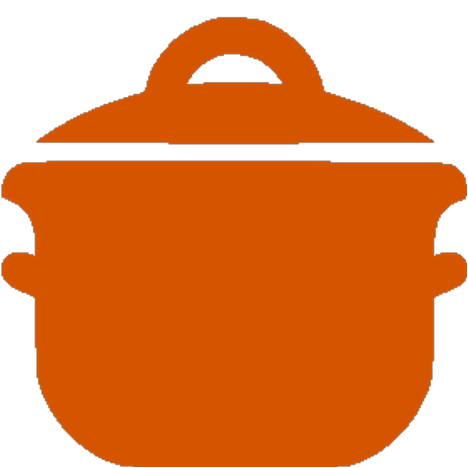
\includegraphics[scale=0.04, trim= 0em -5em -5em -5em,]{Icones/temps_repos_orange.pdf}}
				\parbox{\wd0}{\box0} {#1} \\ 
    \endgroup}
\newcommand{\serve}[1]{
	\begingroup \setbox0=\hbox{
\includegraphics[scale=0.035, trim= 0em -5em -5em -5em,]{Icones/people_281x281_orange.pdf}}
				\parbox{\wd0}{\box0} {#1} \\ 
    \endgroup}

\newcommand{\plogo}{\fbox{$\mathcal{PL}$}} % Generic dummy publisher logo

\newcommand{\showtime}[5]{
	\noindent
	\begin{minipage}[t]{.38\textwidth}
	\vspace{0pt}
	\preptime{ #1 }
	\cooktime{ #2 }
	\chilltime{ #3 }
	\serve{ #4 }
	\end{minipage}		
	\hspace{.02\textwidth}
	\if###5##
    \else
		\begin{minipage}[t]{.6\textwidth}
		\vspace{0pt}
		\includegraphics[width=\linewidth]{#5}%
		\end{minipage}
	\fi
	}

%% Optional argument is the width of the graphic, default = 1in
\newcommand{\showit}[2]{%
    \noindent
	%\begin{minipage}[t]{.38\textwidth}
	\begin{minipage}[t]{\textwidth}
	\vspace{0pt}
	\noindent
	\if###2##
    \else
    	#2
	\fi
  	\end{minipage}
	%\hspace{.02\textwidth}
	%\begin{minipage}[t]{.6\textwidth}
	%\vspace{0pt}
	%\includegraphics[width=\linewidth]{#1}%
  	%\end{minipage}
}
%\newcommand{\forceindent}{\leavevmode{\parindent=1em\indent}}
%\newcommand{\forceindent}{\parindent=1em\indent\parindent=0pt\relax}

%% Optional argument for a  heading within the ingredients section
\newcommand{\ingredients}[1][]{%
    \if###1##%
        {\Large\color{orangecolor}\textbf{Ingredients}}%
    \else
		\emph{#1} :%
    \fi
}
\newcommand{\petitingredients}[1][]{%
    \if###1##%
        {\color{orangecolor}\textbf{Ingredients}}%
    \else
		\emph{#1} :%
    \fi
}

%% Use \obeylines to minimize markup
\newenvironment{petitingreds}{%
	\begin{tcolorbox}[width=\textwidth, breakable,]
 	\parindent0pt
    \noindent
    \petitingredients
    \par
    \medskip

	\setlength{\multicolsep}{0pt}
	\setlength{\columnseprule}{0.5pt}

    \begin{multicols}{2}
    \leftskip0em
    \rightskip0pt plus 3em
    \parskip=0.3em
    \obeylines
    \everypar={\hangindent1em}
	}{%
    \end{multicols}%
	\end{tcolorbox}
}

\newenvironment{ingreds}{%
	\begin{tcolorbox}[width=\textwidth, breakable,]
 	\parindent0pt
    \noindent
    \ingredients
    \par
    \medskip

	\setlength{\multicolsep}{0pt}
	\setlength{\columnseprule}{0.5pt}

    \begin{multicols}{2}
    \leftskip0em
    \rightskip0pt plus 3em
    \parskip=0.3em
    \obeylines
    \everypar={\hangindent1em}
	}{%
    \end{multicols}%
	\end{tcolorbox}
}

\newcounter{stepnum}

%% Optional argument for an italicized pre-step
%% Also use obeylines to minimize markup here as well
\newcommand{\methods}[1][]{%
    \if###1##%
        \parindent0pt
    	\noindent
		{\Large\color{orangecolor}\textbf{Pr\'eparation}}%
		\par
		\vskip 1mm
    \else
        \noindent
     	\normalem
        \emph{#1}%
        \par
	\fi
}

\newenvironment{method}[1][]{%
    \setcounter{stepnum}{0}
    \begingroup
    \parindent0pt
    \parskip0.25em
	\leftskip2em
    \everypar={\llap{\stepcounter{stepnum}\hbox to2em{\thestepnum.\hfill}}}
}{%
    \parskip0.25em
	\par
	\endgroup
	
}
\newenvironment{method_noNumber}[1][]{%
    \setcounter{stepnum}{0}
    \begingroup
    \parindent0pt
    \parskip0.25em
	\leftskip2em
    \everypar={\llap{\hbox to2em{\hfill}}}
}{%
    \par
    \endgroup
	
}

\newenvironment{petitprep}[1][]{%
    \noindent
    {\color{orangecolor}\textbf{Pr\'eparation}}
	\par
	\setcounter{stepnum}{0}
    \begingroup
    \parindent0pt
    \parskip0.25em
	\leftskip2em
    \everypar={\llap{\stepcounter{stepnum}\hbox to2em{\thestepnum.\hfill}}}
}{%
    \par
    \endgroup
	
}
\newcommand{\extra}[1][]{%
	\noindent
	{\textbf{#1}}%
}

\newenvironment{petitprep_noNumber}[1][]{%
    \setcounter{stepnum}{0}
    \begingroup
    \parindent0pt
    \parskip0.25em
	\leftskip2em
    \everypar={\llap{\hbox to2em{\hfill}}}
}{%
    \par
    \endgroup
}

%% Use \obeylines to minimize markup
\newenvironment{vin}[1][]{%
     \if###1##%
     \else
		\begin{minipage}{\textwidth}
		\setcounter{stepnum}{0}
		\noindent
		{\color{orangecolor}\Large\textbf{Vins}}%
		\par
		\medskip
		\parindent20pt
		{#1}
		\end{minipage}
	 \fi
}


%% Use \obeylines to minimize markup
\newenvironment{note}[2][]{%
     \if###1##%
     	\if###2##%
     	\else
			 \begin{tcolorbox}[blanker,width=\textwidth, breakable,]
			 \setcounter{stepnum}{0}
			 \noindent
			 {\color{orangecolor}\Large\textbf{Notes}}%
			 \par
			 \medskip
			 \parindent10pt
			 {#2}
			 \par
			 \smallskip
			 \end{tcolorbox}
		 \fi
	 \else
		 \begin{tcolorbox}[blanker,width=\textwidth, breakable,]
		 \setcounter{stepnum}{0}
		 \noindent
		 {\color{orangecolor}\Large\textbf{Notes}}%
		 \par
		 \medskip
		 \if if###2##%
	     \else
			 \parindent0pt
			 {#2}
			 \par
		 \fi
		 \parindent20pt
		 {#1}
	     \smallskip
		 \end{tcolorbox}
	 \fi
}


\pagestyle{fancy}
% End of "recipes.sty"

\renewcommand{\sectionmark}[1]{\markboth{\MakeUppercase{#1}}{}}
\renewcommand{\subsectionmark}[1]{\markright{#1}{}}


\newcommand*\iconEntree{ 
\checkoddpage
\ifoddpage
	\setbox0=\hbox{\put(-11,7){
\includegraphics[scale=0.017, trim= 0em -5em -5em -5em,]{Icones/icon_entree_white.pdf}}}
	\parbox{\wd0}{\box0}
\else
	\setbox0=\hbox{\put(-14,7){
\includegraphics[scale=0.017, trim= 0em -5em -5em -5em,]{Icones/icon_entree_white.pdf}}}
	\parbox{\wd0}{\box0}
\fi
}
\newcommand*\iconLegume{ 
\checkoddpage
\ifoddpage
	\setbox0=\hbox{\put(-12.,7){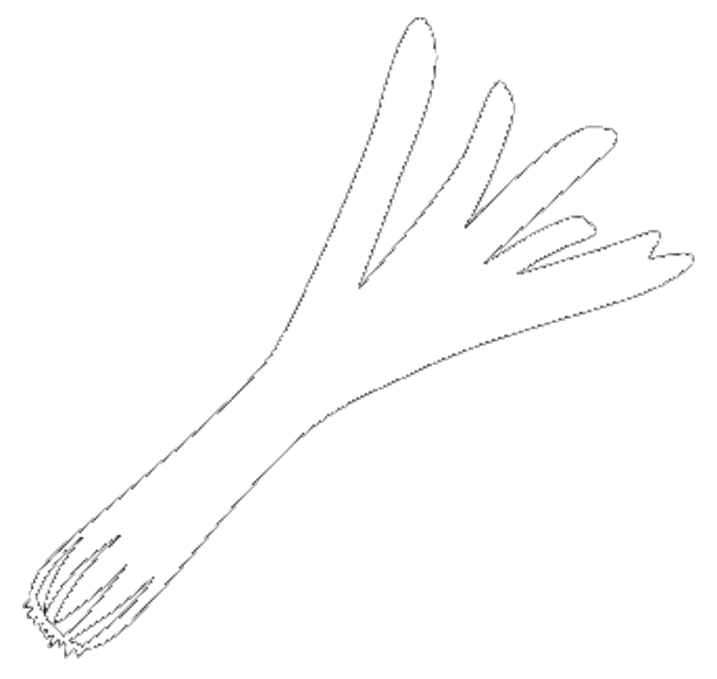
\includegraphics[scale=0.05, trim= 0em -5em -5em -5em,]{Icones/icon_legume_white.pdf}}}
	\parbox{\wd0}{\box0}
\else
	\setbox0=\hbox{\put(-14.5,7){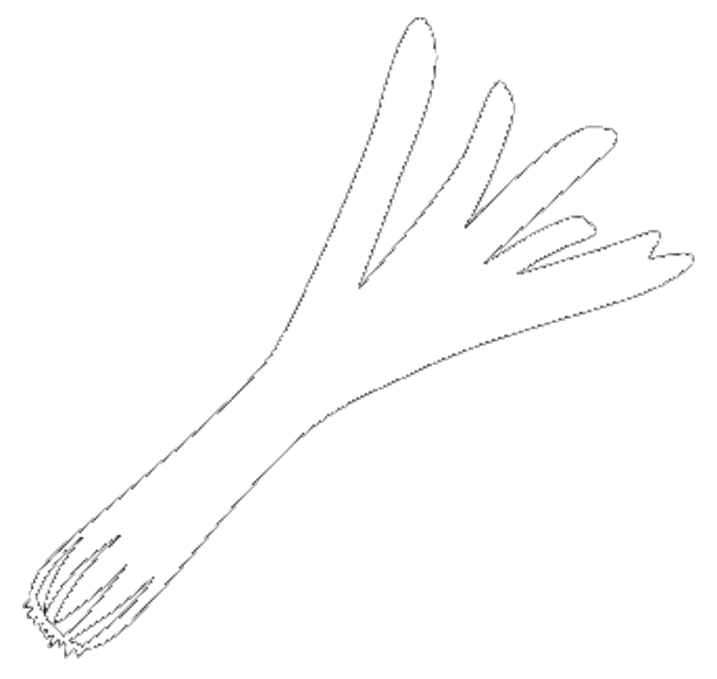
\includegraphics[scale=0.05, trim= 0em -5em -5em -5em,]{Icones/icon_legume_white.pdf}}}
	\parbox{\wd0}{\box0}
\fi
}
\newcommand*\iconPoisson{ 
\checkoddpage
\ifoddpage
	\setbox0=\hbox{\put(-13.5,7){
\includegraphics[scale=0.012, trim= 0em -5em -5em -5em,]{Icones/icon_poisson_white.pdf}}}
	\parbox{\wd0}{\box0}
\else
	\setbox0=\hbox{\put(-15.5,7){
\includegraphics[scale=0.012, trim= 0em -5em -5em -5em,]{Icones/icon_poisson_white.pdf}}}
	\parbox{\wd0}{\box0}
\fi
}
\newcommand*\iconViande{
\checkoddpage
\ifoddpage
	\setbox0=\hbox{\put(-11.7,7){
\includegraphics[scale=0.015, trim= 0em -5em -5em -5em,]{Icones/icon_viande_white.pdf}}}
	\parbox{\wd0}{\box0}
\else
	\setbox0=\hbox{\put(-12.8,7){
\includegraphics[scale=0.015, trim= 0em -5em -5em -5em,]{Icones/icon_viande_white.pdf}}}
	\parbox{\wd0}{\box0}
\fi
}
\newcommand*\iconDessert{ 
\checkoddpage
\ifoddpage
	\setbox0=\hbox{\put(-10.7,8){
\includegraphics[scale=0.016, trim= 0em -5em -5em -5em,]{Icones/icon_dessert_white.pdf}}}
	\parbox{\wd0}{\box0}
\else
	\setbox0=\hbox{\put(-13,8){
\includegraphics[scale=0.016, trim= 0em -5em -5em -5em,]{Icones/icon_dessert_white.pdf}}}
	\parbox{\wd0}{\box0}
\fi
}
\newcommand*\iconSauce{ 
\checkoddpage
\ifoddpage
	\setbox0=\hbox{\put(-11,7){
\includegraphics[scale=0.017, trim= 0em -5em -5em -5em,]{Icones/icon_sauce_white.pdf}}}
	\parbox{\wd0}{\box0}
\else
	\setbox0=\hbox{\put(-12.8,7){
\includegraphics[scale=0.017, trim= 0em -5em -5em -5em,]{Icones/icon_sauce_white.pdf}}}
	\parbox{\wd0}{\box0}
\fi
}

\newcommand*\iconBordeaux{ 
\checkoddpage
\ifoddpage
	\setbox0=\hbox{\put(10,8){
\includegraphics[scale=0.021, trim= 0em -5em -5em -5em,]{Icones/icon_bordeaux_white.pdf}}}
	\parbox{\wd0}{\box0}
\else
	\setbox0=\hbox{\put(0,8){
\includegraphics[scale=0.021, trim= 0em -5em -5em -5em,]{Icones/icon_bordeaux_white.pdf}}}
	\parbox{\wd0}{\box0}
\fi
}

\newcommand*\iconAlsace{ 
\checkoddpage
\ifoddpage
	\setbox0=\hbox{\put(10,8){
\includegraphics[scale=0.021, trim= 0em -5em -5em -5em,]{Icones/icon_alsace_white.pdf}}}
	\parbox{\wd0}{\box0}
\else
	\setbox0=\hbox{\put(0,8){
\includegraphics[scale=0.021, trim= 0em -5em -5em -5em,]{Icones/icon_alsace_white.pdf}}}
	\parbox{\wd0}{\box0}
\fi
}

\newcommand*\iconBourgogne{ 
\checkoddpage
\ifoddpage
	\setbox0=\hbox{\put(10,8){
\includegraphics[scale=0.021, trim= 0em -5em -5em -5em,]{Icones/icon_bourgogne_white.pdf}}}
	\parbox{\wd0}{\box0}
\else
	\setbox0=\hbox{\put(0,8){
\includegraphics[scale=0.021, trim= 0em -5em -5em -5em,]{Icones/icon_bourgogne_white.pdf}}}
	\parbox{\wd0}{\box0}
\fi
}

\newcommand*\iconChampagne{ 
\checkoddpage
\ifoddpage
	\setbox0=\hbox{\put(10,8){
\includegraphics[scale=0.021, trim= 0em -5em -5em -5em,]{Icones/icon_champagne_white.pdf}}}
	\parbox{\wd0}{\box0}
\else
	\setbox0=\hbox{\put(0,8){
\includegraphics[scale=0.021, trim= 0em -5em -5em -5em,]{Icones/icon_champagne_white.pdf}}}
	\parbox{\wd0}{\box0}
\fi
}

\newcommand*\iconJura{ 
\checkoddpage
\ifoddpage
	\setbox0=\hbox{\put(10,8){
\includegraphics[scale=0.021, trim= 0em -5em -5em -5em,]{Icones/icon_jura_white.pdf}}}
	\parbox{\wd0}{\box0}
\else
	\setbox0=\hbox{\put(0,8){
\includegraphics[scale=0.021, trim= 0em -5em -5em -5em,]{Icones/icon_jura_white.pdf}}}
	\parbox{\wd0}{\box0}
\fi
}

\newcommand*\iconLanguedoc{ 
\checkoddpage
\ifoddpage
	\setbox0=\hbox{\put(10,8){
\includegraphics[scale=0.021, trim= 0em -5em -5em -5em,]{Icones/icon_languedoc_white.pdf}}}
	\parbox{\wd0}{\box0}
\else
	\setbox0=\hbox{\put(0,8){
\includegraphics[scale=0.021, trim= 0em -5em -5em -5em,]{Icones/icon_languedoc_white.pdf}}}
	\parbox{\wd0}{\box0}
\fi
}

\newcommand*\iconProvence{ 
\checkoddpage
\ifoddpage
	\setbox0=\hbox{\put(10,8){
\includegraphics[scale=0.021, trim= 0em -5em -5em -5em,]{Icones/icon_provence_white.pdf}}}
	\parbox{\wd0}{\box0}
\else
	\setbox0=\hbox{\put(0,8){
\includegraphics[scale=0.021, trim= 0em -5em -5em -5em,]{Icones/icon_provence_white.pdf}}}
	\parbox{\wd0}{\box0}
\fi
}

\newcommand*\iconSudOuest{ 
\checkoddpage
\ifoddpage
	\setbox0=\hbox{\put(10,8){
\includegraphics[scale=0.021, trim= 0em -5em -5em -5em,]{Icones/icon_sudouest_white.pdf}}}
	\parbox{\wd0}{\box0}
\else
	\setbox0=\hbox{\put(0,8){
\includegraphics[scale=0.021, trim= 0em -5em -5em -5em,]{Icones/icon_sudouest_white.pdf}}}
	\parbox{\wd0}{\box0}
\fi
}

\newcommand*\iconLoire{ 
\checkoddpage
\ifoddpage
	\setbox0=\hbox{\put(10,8){
\includegraphics[scale=0.021, trim= 0em -5em -5em -5em,]{Icones/icon_loire_white.pdf}}}
	\parbox{\wd0}{\box0}
\else
	\setbox0=\hbox{\put(0,8){
\includegraphics[scale=0.021, trim= 0em -5em -5em -5em,]{Icones/icon_loire_white.pdf}}}
	\parbox{\wd0}{\box0}
\fi
}

\newcommand*\iconRhone{ 
\checkoddpage
\ifoddpage
	\setbox0=\hbox{\put(10,8){
\includegraphics[scale=0.021, trim= 0em -5em -5em -5em,]{Icones/icon_rhone_white.pdf}}}
	\parbox{\wd0}{\box0}
\else
	\setbox0=\hbox{\put(0,8){
\includegraphics[scale=0.021, trim= 0em -5em -5em -5em,]{Icones/icon_rhone_white.pdf}}}
	\parbox{\wd0}{\box0}
\fi
}

\def\Entrees{ Entrées}
\def\Legumes{ Plats de L\'egume}
\def\Poissons{ Plats de Poisson}
\def\Viandes{ Plats de Viande}
\def\Desserts{ Desserts}
\def\Sauces{ Sauces et Condiments}

\def\Bordeaux{ Bordeaux}
\def\Alsace{ Alsace}
\def\Bourgogne{ Bourgogne}
\def\Champagne{ Champagne}
\def\Jura{ Jura}
\def\Languedoc{ Languedoc-Roussillon}
\def\Provence{ Provence}
\def\SudOuest{ Sud-Ouest}
\def\Loire{ Vall\'ee de la Loire}
\def\Rhone{ Vall\'ee du Rhône}



\newcommand*{\subsectionnumber}{\arabic{subsection}}

\makeatletter
\newcommand\testCat[2]{%
 %\texttt{\string\myoldvalue}: \myoldvalue\\
 %ARG1: #1\\
 \ifnum\pdf@strcmp{#2}{#1}=\z@
   0%
 \else
   1%
 \fi
}
\makeatother

\newcommand*{\thumbsIcon}{
	\ifnum0=\subsectionnumber\relax
	%	
	\fi
	\ifnum0=\testCat{\currentSectionName}{\Entrees}
	%\ifnum1=\subsectionnumber\relax 
	\iconEntree
	\fi
	\ifnum0=\testCat{\currentSectionName}{\Legumes}
	\iconLegume
	\fi
	%\ifnum2=\subsectionnumber\relax
	\ifnum0=\testCat{\currentSectionName}{\Poissons}
	\iconPoisson
	\fi
	%\ifnum3=\subsectionnumber\relax
	\ifnum0=\testCat{\currentSectionName}{\Viandes}
	\iconViande
	\fi
	%\ifnum4=\subsectionnumber\relax
	\ifnum0=\testCat{\currentSectionName}{\Desserts}
	\iconDessert
	\fi
	\ifnum0=\testCat{\currentSectionName}{\Sauces}
	%\ifnum5=\subsectionnumber\relax
	\iconSauce
	\fi
	
	\ifnum0=\testCat{\currentSectionName}{\Bordeaux}
	%\ifnum1=\subsectionnumber\relax 
	\iconBordeaux
	\fi
	
	\ifnum0=\testCat{\currentSectionName}{\Alsace}
	%\ifnum1=\subsectionnumber\relax 
	\iconAlsace
	\fi
	
	\ifnum0=\testCat{\currentSectionName}{\Bourgogne}
	%\ifnum1=\subsectionnumber\relax 
	\iconBourgogne
	\fi
	
	
	\ifnum0=\testCat{\currentSectionName}{\Champagne}
	%\ifnum1=\subsectionnumber\relax 
	\iconChampagne
	\fi
	
	\ifnum0=\testCat{\currentSectionName}{\Jura}
	%\ifnum1=\subsectionnumber\relax 
	\iconJura
	\fi
	
	\ifnum0=\testCat{\currentSectionName}{\Languedoc}
	%\ifnum1=\subsectionnumber\relax 
	\iconLanguedoc
	\fi
	
	\ifnum0=\testCat{\currentSectionName}{\Provence}
	%\ifnum1=\subsectionnumber\relax 
	\iconProvence
	\fi
	
	\ifnum0=\testCat{\currentSectionName}{\SudOuest}
	%\ifnum1=\subsectionnumber\relax 
	\iconSudOuest
	\fi
	
	\ifnum0=\testCat{\currentSectionName}{\Loire}
	%\ifnum1=\subsectionnumber\relax 
	\iconLoire
	\fi

	\ifnum0=\testCat{\currentSectionName}{\Rhone}
	%\ifnum1=\subsectionnumber\relax 
	\iconRhone
	\fi

	}

\newcommand*{\currentSectionName}{
	\ifnum0=\subsectionnumber\relax
	%	
	\else
	\Subsectionname
	\fi
	}
\let\Subsectionmark\subsectionmark
\def\subsectionmark#1{\def\Subsectionname{#1}\Subsectionmark{#1}}



%%%%%%%%%%%%%%%%%%%%%%%%%%%%%%%%%%
\begin{document}
%%%%%%%%%%%%%%%%%%%%%%%%%%%%%%%%%%

\pagenumbering{arabic}

\begin{titlepage} % Suppresses headers and footers on the title page
	
	\centering % Centre everything on the title page
	
	%------------------------------------------------
	%	Top rules
	%------------------------------------------------
	
	\rule{\textwidth}{1pt} % Thick horizontal rule
	
	\vspace{2pt}\vspace{-\baselineskip} % Whitespace between rules
	
	\rule{\textwidth}{0.4pt} % Thin horizontal rule
	
	\vspace{0.1\textheight} % Whitespace between the top rules and title
	
	%------------------------------------------------
	%	Title
	%------------------------------------------------
	\color{orangecolor}{	
	{\Huge Les Recettes}\\[0.5\baselineskip] % Title line 1
	{\Large de}\\[0.5\baselineskip] % Title line 2
	{\Huge Coat Tanguy} % Title line 3
	}
	\color{black}	
	\vspace{0.025\textheight} % Whitespace between the title and short horizontal rule
	
	\rule{0.3\textwidth}{0.4pt} % Short horizontal rule under the title
	
	\vspace{0.1\textheight} % Whitespace between the thin horizontal rule and the author name
	
	%------------------------------------------------
	%	Author
	%------------------------------------------------
	
	{\Large \textsc{Renee et Jean Paul Paugam}} % Author name
	
	\vfill % Whitespace between the author name and publisher
	
	%------------------------------------------------
	%	Publisher
	%------------------------------------------------

	{
\includegraphics[scale=1.]{tourBlanche_calque-seul}}
	
	{\large\textsc{Gwelet Veo Edition}} % Publisher
	
	\vspace{0.1\textheight} % Whitespace under the publisher text
	
	%------------------------------------------------
	%	Bottom rules
	%------------------------------------------------
	\color{black}
	\rule{\textwidth}{0.4pt} % Thin horizontal rule
	
	\vspace{2pt}\vspace{-\baselineskip} % Whitespace between rules
	
	\rule{\textwidth}{1pt} % Thick horizontal rule
	
\end{titlepage}

%############

\clearpage % end title page
\begingroup
  \pagestyle{empty}
  \null
  \newpage
\endgroup

\frontmatter

\section*{Avant Propos}
Les souvenirs de famille peuvent être une formidable source d’énergie. Ils ne sont pas un simple retour du passé. Ils constituent notre identité. Le socle commun des souvenirs est la trame des liens familiaux : les valeurs, les convictions, les histoires, les faits marquants du passé familial et les rites que tout le monde partage. Parmi ces rites, figurent en première place les recettes de cuisine.

Une recette de cuisine, ce n’est pas qu’une photo dans un livre ou sur un site internet accompagnée d’un algorithme qu’on veut, le plus souvent, vous faire passer pour le plus simple possible pour ne pas vous décourager \ldots~ Non, une recette de cuisine c’est tout d’abord la promesse de passer quelques heures entre l’évier, la plaque de cuisson, le four et le frigo à éplucher, découper, parer, laver, égoutter, essorer, mélanger, battre, cuire, remuer, goûter, présenter. C’est aussi, au bout du compte, le plaisir de régaler sa famille et ses amis. Si, de plus, ces recettes sont celles que l’on s’est passées de génération en génération, elles ont inévitablement le pouvoir de faire revenir des souvenirs que les odeurs et les saveurs peuvent réveiller. Tout le monde a sa madeleine\ldots

\textit{« Et tout d'un coup le souvenir m'est apparu. Ce goût c'était celui du petit morceau de madeleine que le dimanche matin, à Combray (parce que ce jour-là je ne sortais pas avant l'heure de la messe), quand j'allais lui dire bonjour dans sa chambre, ma tante Léonie m'offrait après l'avoir trempé dans son infusion de thé ou de tilleul. [\ldots] Quand d'un passé ancien rien ne subsiste, après la mort des êtres, après la destruction des choses, seules, plus frêles mais plus vivaces, plus immatérielles, plus persistantes, plus fidèles, l'odeur et la saveur restent encore longtemps, comme des âmes, à se rappeler, à attendre, à espérer, sur la ruine de tout le reste, à porter sans fléchir, sur leur gouttelette presque impalpable, l'édifice immense du souvenir. »} Marcel Proust, A la recherche du temps perdu, 1913

C’est Ronan qui a souhaité, dans un premier temps, réunir sur un site nos archives familiales (généalogie, chansons, poèmes, recettes)\footnote{\url{http://paugam.info/}}. Ensuite pour en faire plus profiter la famille et les amis, et en fin gastronome, il a décidé de faire une version imprimée des recettes. 
%Mettant à profit son expertise dans le codage informatique, il a créé le cadre du site puis la maquette de ce « cookbook » et joué le rôle du chef de rédaction.
      
Nous avons donc rassemblé dans ces pages toutes les recettes que nous mettons en œuvre pour garnir notre table au quotidien ou pour les jours de fête. Elles sont rangées dans 4 chapitres : Famille, Bretagne, Maroc et Autriche.

Le chapitre « Famille » regroupe les plats issus de notre tradition culinaire familiale. Si la cuisine de Saint-Pierre-Quilbignon ou celle de Ploudaniel ont été le lieu de nos premières armes, notre cuisine familiale s’est aussi enrichie au gré de nos rencontres.

Un chapitre « Bretagne » a été consacré aux recettes de cette région parce que, bretons, cette cuisine fait partie de notre culture, de notre identité. Préparés à partir des produits locaux de la terre et de la mer, certains de ces plats sont traditionnels et d’autres sont le fruit de la rencontre de la nouvelle cuisine avec notre terroir.

Le chapitre « Maroc » est le recueil des recettes de ce pays où nous avons passé 13 ans. Pendant ce séjour, grâce à Halima et Rkia, nos deux bonnes, nous avons pu apprécier cette cuisine riche, délicate et parfumée.

Le chapitre « Autriche » a été rédigé par Maëlle qui a passé 2 ans à Vienne. Elle a découvert la gastronomie autrichienne qui est une bonne synthèse de toutes les cuisines d’Europe Centrale et elle a surtout apprécié la pâtisserie viennoise. 

Un dernier chapitre est consacré à la cave que Jean Paul a constitué d’année en année avec l’aide d’amis, comme lui, amateurs de bons vins. Il assume le rôle de sommelier en cherchant les meilleurs accords mets et vins. Mais à notre table, pas de grands principes et de méthodes sophistiquées de dégustation, le vin est apprécié comme le produit tel qu’il est et à l’aune du plaisir qu’il permet de partager. Pour chaque recette, nous avons donc indiqué le choix de vins que Jean Paul a sélectionné dans sa cave pour accompagner le plat.

Nous vous souhaitons de belles aventures dans votre cuisine et un bon appétit en bonne compagnie.

\vspace{16pt}
\hfill
\parbox{2cm}{
Renée. 
}

%############

\newpage
\fancyhead{} % clear all header fields
\fancyhead[LE]{\bfseries\nouppercase{\leftmark}}      % Chapter in the right on even pages
\fancyhead[RO]{\bfseries\nouppercase{\leftmark}}      % Chapter in the right on even pages
\tableofcontents

\newpage
\fancyhead{}
\fancyhead[LE]{\bfseries\nouppercase{Tables des Icônes}}      % Chapter in the right on even pages
\fancyhead[RO]{\bfseries\nouppercase{\leftmark}}      % Chapter in the right on even pages


\section*{Marques et Icônes} 

\subsection*{Chapitres}
A droite ou à gauche de chaque page selon qu’elle soit paire ou impaire, se trouve une marque de couleur se référant à chaque chapitre.
Le code couleur est défini sur la page de droite.

Dans chaque chapitre, les recettes sont réunies dans différentes rubriques symbolisées par une icônes qui 
apparait dans la marque de couleur :
\vskip 2mm
{\renewcommand{\arraystretch}{1.7}
\begin{tabular}[!h]{ l l }
\setbox0=\hbox{\put(0,0){
\includegraphics[scale=0.013, trim= 0em -5em -5em -5em,]{Icones/icon_entree_black.pdf}}}
	\parbox{\wd0}{\box0} 
	& \quad Entrées  \\ 
\setbox0=\hbox{\put(-3,0){
\includegraphics[scale=0.05, trim= 0em -5em -5em -5em,]{Icones/icon_legume_black.pdf}}}
	\parbox{\wd0}{\box0}
	& \quad Plats de L\'egume  \\ 
\setbox0=\hbox{\put(-4,0){
\includegraphics[scale=0.012, trim= 0em -5em -5em -5em,]{Icones/icon_poisson_black.pdf}}}
	\parbox{\wd0}{\box0}
	& \quad Plats de Poisson  \\ 
\setbox0=\hbox{\put(0,0){
\includegraphics[scale=0.013, trim= 0em -5em -5em -5em,]{Icones/icon_viande_black.pdf}}}
	\parbox{\wd0}{\box0}
	& \quad Plat de Viande  \\ 
	\setbox0=\hbox{\put(0,0){
\includegraphics[scale=0.014, trim= 0em -5em -5em -5em,]{Icones/icon_dessert_black.pdf}}}
	\parbox{\wd0}{\box0}
	& \quad Dessert  \\ 
\setbox0=\hbox{\put(0,0){
\includegraphics[scale=0.014, trim= 0em -5em -5em -5em,]{Icones/icon_sauce_black.pdf}}}
	\parbox{\wd0}{\box0}
	& \quad Sauce de Accompagnement  \\ 
\end{tabular}
}

\subsection*{Recettes}
Dans chaque recette, sont données des informations de temps et de service. Elles sont indiquées par les icônes ci-dessous : 
\vskip 2mm
\begin{tabular}{ l l }
\setbox0=\hbox{
\includegraphics[scale=0.05, trim= 0em -5em -5em -5em,]{Icones/temps_preparation_orange.pdf}} \parbox{\wd0}{\box0}  
	& temps de pr\'eparation  \\ 
\setbox0=\hbox{
\includegraphics[scale=0.05, trim= 0em -5em -5em -5em,]{Icones/temps_cuisson_orange.pdf}} \parbox{\wd0}{\box0}  
	& temps de cuisson  \\ 
\setbox0=\hbox{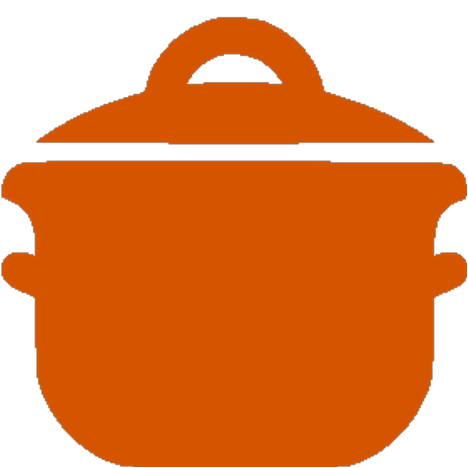
\includegraphics[scale=0.05, trim= 0em -5em -5em -5em,]{Icones/temps_repos_orange.pdf}} \parbox{\wd0}{\box0}  
	& temps de repos  \\ 
\setbox0=\hbox{
\includegraphics[scale=0.05, trim= 0em -5em -5em -5em,]{Icones/people_281x281_orange.pdf}} \parbox{\wd0}{\box0}  
	& nombre de services  \\ 
\end{tabular}

Les chiffres entre crochets indiquent des r\'ef\'erences bibliographiques qui ont
inspir\'ees certaines recettes. Ces r\'ef\'erences sont list\'ees page \pageref{sec:references}.

%############

%\addthumbsoverviewtocontents{section}{Table des Marques de Couleurs}%
\thumbsoverview{Les Marques de Chapitres}

\newpage
\fancyhead{}

\mainmatter
\setcounter{page}{1}

%XX
\section{Famille}                                          
\addthumb{Famille}{\thumbsIcon}{white}{jade}
On ne se nourrit pas seulement de plats plus ou moins sophistiqués mais aussi d'émotions… Quoi de mieux que les odeurs et le goût de la cuisine de notre enfance pour revivre des moments agréables. Pourquoi le parfum de la viande qui crépite dans le beurre au fond de la cocotte avant de cuire en ragoût fait remonter à la mémoire le goût du café au lait ?$\ldots$ Parce que le jeudi, jour où il n’y avait pas d’école, on se levait plus tard et on prenait son petit déjeuner dans la cuisine où maman commençait déjà la préparation du repas de midi$\ldots$
Dans notre famille, chaque génération a laissé son empreinte dans la tradition
culinaire. Elle s’est construite à partir des habitudes gastronomiques, des
voyages et des rencontres de chacun. Les recettes, qui en sont l’expression, sont
regroupées dans ce chapitre intitulé « Famille ». Il y a les recettes héritées de
Grand-Mère Saint-Pierre qui se faisait un point d’honneur de pratiquer la
cuisine bourgeoise en toute rigueur suivant les canons de H.P.
Pellaprat \cite{pellaprat} et de réaliser avec la même rigueur les plats traditionnels des pays et régions où elle avait séjourné. Grand-Mère Ploudaniel, quant à elle, nous a laissé les goûteuses recettes qu’elle préparaient avec les produits du jardin, pommes de terre, échalotes, rhubarbe sans oublier les lapins de ses clapiers. Notre cuisine familiale s’est aussi enrichie de partage entre frères et sœurs et la nouvelle génération a introduit la notion de cuisine flexitarienne et donné le grade de « plat » aux légumes qui n’avaient jusque-là qu’un rôle de « garniture ».

\newpage

\section{Bretagne}                                          
\addthumb{Bretagne}{\thumbsIcon}{white}{glaucous}
La cuisine bretonne n’est pas faite que de crêpes, de kig-ha-farz ou de kouign-amann. Elle est bien plus riche et, avant tout, elle fait partie de notre culture et notre identité. Elle représente notre terroir parce qu’elle est le fruit de la rencontre des ressources naturelles, produits locaux agricoles et de la pêche, avec un peuple, ses us, ses coutumes et ses croyances. Il y a la cuisine des campagnes (argoat) et celle de la côte (armor), la cuisine de fête et celle de tous les jours. Si les recettes traditionnelles sont toujours scrupuleusement préparées, la nouvelle cuisine s’est aussi approprié ces ressources pour en faire des plats nouveaux.
Ce chapitre « Bretagne » est consacré aux recettes transmises de mère en fille et en fils à Saint-Pierre, à Ploudaniel et à Coat Tanguy. Leur liste s’enrichit maintenant au gré des repas de famille ou de ceux partagés avec des amis bretons. Dans plusieurs de ces recettes, les ingrédients sont importants mais ce qui l’est encore plus ce sont les tours de main que Grand-Mère Saint-Pierre comme Grand-Mère Ploudaniel se faisaient un devoir et un plaisir de nous enseigner.

\newpage

\section{Maroc}                                          
\addthumb{Maroc}{\thumbsIcon}{white}{antiquebrass}
Le Maroc est le pays où nous avons passé 13 ans. Pendant ce séjour, nous avons eu deux bonnes, Halima et Rkia. Grâce à elles, nous avons réussi à nous adapter aux us et coutumes de ce pays et en comprendre les subtilités. Halima s’occupa de notre maison, à Rabat, de 1975 à 1980. C’était une vieille dame délicieuse qui avait travaillé dans les cuisines d’un ministère et qui était donc une excellente cuisinière. Rkia, quant à elle, partagea notre quotidien de 1980 à 1988, à Rabat après le décès de Halima, puis à Agadir. Elle était toute jeune, très curieuse et prête à toutes les expériences culinaires.
Ce chapitre « Maroc » est donc le recueil de leurs recettes. Elles nous ont préparé tous ces plats avec tant de plaisir et de générosité. Pendant ces treize années, elles ont eu le souci de nous faire découvrir toutes les richesses de la cuisine marocaine si parfumée et délicate. Aujourd’hui, les odeurs et le goût d’un « tagine » nous rappellent l’ambiance des souks, des repas pantagruéliques chez les collègues marocains, des restaurants de palace comme de ceux du fin fond du bled.

\newpage

\section{Autriche}                                          
\addthumb{Autriche}{\thumbsIcon}{white}{manatee}
Chaque génération a connu ses émigrations. Pour des raisons professionnelles ou d’études, elles ont permis de découvrir d’autres cultures aux quatre coins de la France ou à l’étranger. Après l’Indochine, l’Algérie, les rives de la Méditerranée, la Picardie et l’Anjou pour les grands-parents, le Maroc pour les parents baby-boomers, les enfants de la génération Y se sont exilés dans les pays anglo-saxons ou germaniques (la Grande Bretagne et les Etats-Unis pour Ronan, l’Autriche pour Maëlle).
Si Ronan a surtout choisi le rôle de critique gastronomique, Maëlle s’est essayée avec bonheur à la cuisine autrichienne. Etudiante ERASMUS à Vienne pendant 2 ans et très intéressée et douée pour la pâtisserie, outre un diplôme d’ingénieure, elle a rapporté de ce séjour les recettes regroupées dans ce dernier chapitre « Autriche ». On y trouve certains plats traditionnels mais surtout les fameux gâteaux qui font la réputation des cafés viennois. Stefan Zweig écrit dans ses mémoires (Le Monde d’Hier) : « Le Kaffeehaus représente une institution d'un genre particulier, qui ne peut être comparée à aucune autre au monde. »

\newpage

\newcommand{\vinSection}[2][\newpage]{%
	#1
	\fancyhead[LE]{\bfseries\nouppercase{\leftmark}}      % Chapter in the right on even pages
	\fancyhead[RO]{\bfseries\nouppercase{\leftmark}}      % Chapter in the right on even pages
	\fancyhead[LO]{\bfseries\nouppercase{\rightmark}}      % Chapter in the right on even pages
	\fancyhead[RE]{\bfseries\nouppercase{\rightmark}}      % Chapter in the right on even pages
	%\lhead{\leftmark}%
    \chead{}%
    %\rhead{\rightmark}%
    \lfoot{}%
    \rfoot{}%
    \subsubsection{#2}%
}


\newcommand{\vinShowInfoDomain}[3]{
	\noindent
	\begin{minipage}[t]{\textwidth}
	\vspace{0pt}
		\begin{tabular}{l p{7.5cm} }
		Producteur:     & {#1}\\
		Adresse:        & {#2}\\
	\end{tabular}
	\end{minipage}		
	\par
	\hfill
	\vspace{2pt}
	\begin{figure}[!h]
		\includegraphics[width=\textwidth]{#3}
	\end{figure}
	}
\newcommand{\vinShowCouleur}[1]{
	\noindent
	\begin{minipage}[t]{.3\textwidth}
	%\begin{tcolorbox}[width=.3\textwidth,]
		{\color{orangecolor}\textbf{#1}}
	%\end{tcolorbox}
	\end{minipage}	
	\hfill
	\vspace{6pt}
	}

\newcommand{\vinShowInfoAppellation}[3]{
	\noindent
	\begin{minipage}[t]{\textwidth}
	{\textbf{#1}}%
	\vspace{1pt}
	\end{minipage}		
	\begin{minipage}[t]{\textwidth}
		\begin{tabular}{l p{7.5cm} }
		Cuv\'ee :    & {#2}\\ 
		C\'epage:    & {#3}\\
	\end{tabular}
	\end{minipage}		
	}

\setlength{\ellipsisgap}{0.02em}

%%%%%%%%%%%%%%%%%%%%%%%%%%%%%%%%%%%

\newpage 
\fancyhead[LE]{\bfseries\nouppercase{\leftmark} } 
\fancyhead[RO]{\bfseries\nouppercase{\leftmark} } 
\fancyhead[LO]{\bfseries\nouppercase{\rightmark} }
\fancyhead[RE]{\bfseries\nouppercase{\rightmark} }

\section{Au Sujet des Vins}
\addthumb{Au Sujet des Vins}{\thumbsIcon}{white}{darkraspberry}

Peut-on imaginer de servir un repas sans l’accompagner de boissons choisies pour en sublimer les saveurs ? Il est donc important de trouver les accords mets/vins les plus appropriés. Il faut remarquer que les goûts et les odeurs ne pouvant être qualibrés par une grandeur physique (contrairement aux couleurs et aux bruits), il n’existe pas de vocabulaire précis pour les qualifier et leur appréciation est essentiellement subjective.
Pour accorder les goûts des plats et des vins, il y a bien quelques principes de sommelier en la matière, mais la meilleure solution reste la dégustation et le partage des sensations entre convives.
Jean Paul a rassemblé dans sa cave des vins en provenance des différents bassins viticoles de France et quelques crus étrangers. Ces vins ont été découverts grâce à des dégustations entre amis ou à l’occasion de visites de salons.
Dans ce chapitre, les vins sont rangés par bassin (ou région). Chaque bassin est symbolisé par une icône qui apparait dans la vignette de couleur. Le symbole représente la forme du verre caractéristique du vignoble.
\medskip
{\renewcommand{\arraystretch}{1.7}
\begin{center}
\begin{tabular}{ l l l l }
\setbox0=\hbox{\put(0,0){\includegraphics[scale=0.021, trim= 0em -5em -5em -5em,]{Icones/icon_alsace_black.pdf}}}
	\parbox{\wd0}{\box0} 
	& \quad Alsace  & 
\setbox0=\hbox{\put(0,0){\includegraphics[scale=0.021, trim= 0em -5em -5em -5em,]{Icones/icon_bordeaux_black.pdf}}}
	\parbox{\wd0}{\box0}
	& \quad Bordeaux  \\ 
\setbox0=\hbox{\put(0,0){\includegraphics[scale=0.021, trim= 0em -5em -5em -5em,]{Icones/icon_bourgogne_black.pdf}}}
	\parbox{\wd0}{\box0}
	& \quad Bourgogne  & 
\setbox0=\hbox{\put(0,0){\includegraphics[scale=0.021, trim= 0em -5em -5em -5em,]{Icones/icon_champagne_black.pdf}}}
	\parbox{\wd0}{\box0}
	& \quad Champagne  \\ 
\setbox0=\hbox{\put(0,0){\includegraphics[scale=0.021, trim= 0em -5em -5em -5em,]{Icones/icon_jura_black.pdf}}}
	\parbox{\wd0}{\box0}
	& \quad Jura  & 
\setbox0=\hbox{\put(0,0){\includegraphics[scale=0.021, trim= 0em -5em -5em -5em,]{Icones/icon_languedoc_black.pdf}}}
	\parbox{\wd0}{\box0}
	& \quad Languedoc-Rousillon  \\ 
\setbox0=\hbox{\put(0,0){\includegraphics[scale=0.021, trim= 0em -5em -5em -5em,]{Icones/icon_provence_black.pdf}}}
	\parbox{\wd0}{\box0}
	& \quad Provence  & 
\setbox0=\hbox{\put(0,0){\includegraphics[scale=0.021, trim= 0em -5em -5em -5em,]{Icones/icon_sudouest_black.pdf}}}
	\parbox{\wd0}{\box0}
	& \quad Sud-Ouest \\ 
\setbox0=\hbox{\put(0,0){\includegraphics[scale=0.021, trim= 0em -5em -5em -5em,]{Icones/icon_loire_black.pdf}}}
	\parbox{\wd0}{\box0}
	& \quad Vallée de la Loire  & 
\setbox0=\hbox{\put(0,0){\includegraphics[scale=0.021, trim= 0em -5em -5em -5em,]{Icones/icon_rhone_black.pdf}}}
	\parbox{\wd0}{\box0}
	& \quad Vallée du Rhône  \\ 
\end{tabular}
\end{center}
}
\medskip
Un verre à vin est un verre à pied et doit être manipulé en le tenant par ce pied afin que la température du vin ne soit pas perturbée par la main. Par ailleurs, chaque vin doit être dégusté à une certaine température. Plus le vin doit rester frais, plus le pied du verre sera haut et le réservoir petit (Alsace, Loire, Champagne). Pour les vins qui ont en majorité des arômes légers qui s’évaporent vites (vins jeunes, Provence, Sud-Ouest, Languedoc-Roussillon), le bord du verre doit être resserré pour que le nez ait le temps de les apprécier. Pour les vins qui ont en majorité des arômes lourds (Jura), le bord sera large pour favoriser l’oxygénation qui fait remonter ces arômes. L’oxygénation sera aussi favorisée dans un verre à fond rond dans lequel on peut faire tourner le vin (vieux vins, Bordeaux, Rhône). Pour des vins plus complexes (Bourgogne), un bord resserré piègera les arômes légers et le fond rond permettra de faire remonter les arômes lourds.  
La carte des bassins viticoles de France est présentée ci-dessous.
\begin{figure}[!t]
\includegraphics[width=\textwidth]{./VinMaps/bassinViticoleFrance.png}
\end{figure}
\newpage
Pour chaque bassin, sont ensuite répertoriés les châteaux ou domaines et leur proposition d’AOP (Appellations d’Origine Protégée qui remplacent les AOC, Appellation d’Origine Contrôlée) et d’IGP (Indications Géographiques Protégées). Leurs cépages sont rapportés lorsque le producteur les a précisés. Les coordonnées de ce dernier sont également indiquées.     

%############

XX



%############

\end{document}
